\section{Experimental Evaluation}\label{sec:evaluation}

\subsection{Evaluation Design and Testbed}
The evaluation combines (i)~a functional validation campaign over the full enrollment-to-deployment path and (ii)~a sustainability-oriented measurement pass on the same test bed. The functional study asks whether cloud intent, gateway mediation, and embedded WASM execution produce mutually consistent evidence under repeatable conditions. The sustainability pass quantifies southbound wire sizes, edge firmware footprint, and Kubernetes pod resource use. Neither pass claims measured joules or carbon reductions; they establish baselines relevant to green-experimentation follow-up.

Experiments run on a single-node K3s cluster with API server, gateway, application controller, and CRDs active. The southbound endpoint is a Renode-emulated STM32F746 running Zephyr firmware with WAMR; it connects over TAP-based networking with DNAT to the gateway TLS port. Table~\ref{tab:testbed} summarizes the host and software stack.

\begin{table}[t]
\centering
\caption{Experimental testbed and software configuration.}
\label{tab:testbed}
\footnotesize
\setlength{\tabcolsep}{3pt}
\begin{tabular}{p{0.30\linewidth} p{0.62\linewidth}}
\toprule
\textbf{Item} & \textbf{Configuration} \\
\midrule
Host OS & Ubuntu 24.04 LTS (kernel 6.8.0), x86\_64 KVM guest \\
Host resources & 32 vCPUs, 62~GiB RAM, 293~GiB SSD \\
Orchestrator & K3s v1.35.4+k3s1, single control-plane node \\
Southbound emulation & Renode \texttt{antmicro/renode:nightly}, board \texttt{Stm32F746gDisco} \\
Firmware stack & Zephyr RTOS 3.5.0, WAMR 2.4.1, minimal WASM test module (33~B) \\
Device networking & TAP \texttt{tap0} at 192.168.1.1/24, DHCP, DNAT to gateway TLS on port 30443 \\
\bottomrule
\end{tabular}
\end{table}

After one warm-up run, the campaign executes $n{=}100$ independent trials. Each trial performs enrollment verification, heartbeat supervision, and deployment of the minimal WASM module to the same emulated device. A trial is \emph{transactionally} successful only if all three stages succeed and deployment evidence is consistent across the gateway runtime view and the Application CRD (\texttt{phase=Running}, device connected, fresh heartbeat). Continuous latencies use monotonic client-side timers; we report mean, standard deviation, median, p95, p99, IQR, CV, and 95\% CI of the mean ($\bar{x} \pm t_{0.975,n-1}\,s/\sqrt{n}$, with $t_{0.975,99}{=}1.984$). For binary outcomes we use Wilson score intervals; with 100/100 successes the 95\% lower bound is 96.3\%.

\subsection{Functional Validation Results}
All 100 transactional trials completed successfully: enrollment, heartbeat supervision, deployment, and cross-layer evidence checks never failed. Because every stage shares the same flawless outcome, a per-stage success table would repeat identical Wilson bounds and is omitted; the meaningful variation lies in latency and its distribution.

Table~\ref{tab:quantitative-latency} reports the latency profile. Mean end-to-end latency (enrollment plus deployment; heartbeat excluded as a sub-millisecond probe) is 1185.8~ms with 95\% CI [1152.8, 1218.7]~ms. The heartbeat row reflects \emph{observability} latency---how quickly the measurement harness reads a fresh heartbeat from the gateway---not the 25~s firmware emission interval.

\begin{table}[t]
\centering
\caption{Latency profile ($n{=}100$ trials). All values in milliseconds.}
\label{tab:quantitative-latency}
\footnotesize
\setlength{\tabcolsep}{2pt}
\resizebox{\columnwidth}{!}{%
\begin{tabular}{lrrrrrrr}
\toprule
\textbf{Stage} & \textbf{Mean} & \textbf{Median} & \textbf{p95} & \textbf{p99} & \textbf{IQR} & \textbf{CV} & \textbf{95\% CI of mean} \\
\midrule
Enrollment & 583.9 & 557.4 & 773.4 & 791.1 & 58.8 & 0.142 & [567.5, 600.3] \\
Heartbeat obs. & 4.43 & 4.31 & 5.79 & 7.05 & 0.73 & 0.153 & [4.30, 4.57] \\
Deployment & 601.9 & 542.8 & 1031.3 & 1295.7 & 88.0 & 0.288 & [567.5, 636.3] \\
End-to-end & 1185.8 & 1132.5 & 1561.1 & 1789.6 & 191.5 & 0.140 & [1152.8, 1218.7] \\
\bottomrule
\end{tabular}%
}
\end{table}

Figure~\ref{fig:latency-boxplot} compares stage latency distributions on a logarithmic scale. Heartbeat observability is two orders of magnitude faster than enrollment or deployment. Figure~\ref{fig:latency-cdf} shows that deployment contributes most of the tail mass: its p95 (1031.3~ms) and p99 (1295.7~ms) exceed enrollment's, so WASM orchestration---not TLS enrollment---dominates end-to-end variability (deployment CV\,=\,0.288 vs.\ enrollment CV\,=\,0.142).

\begin{figure}[!htbp]
\centering
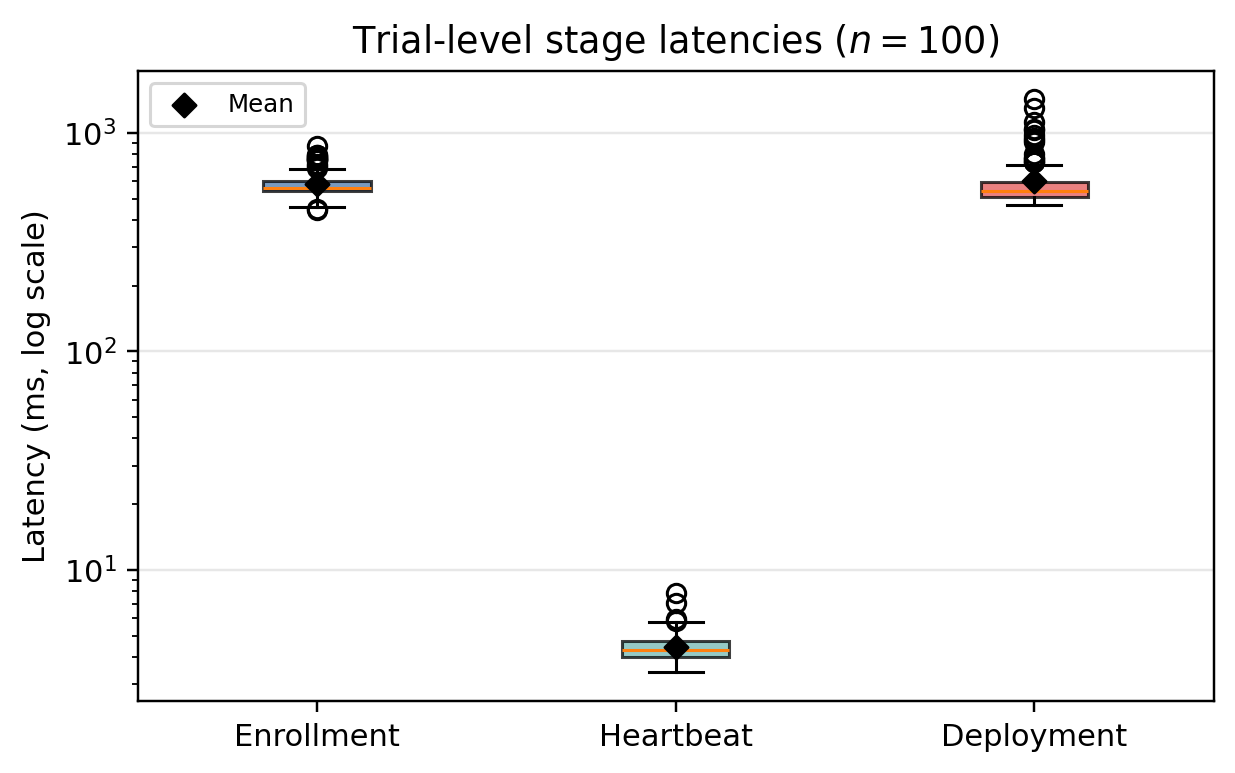
\includegraphics[width=\columnwidth,height=0.26\textheight,keepaspectratio]{figures/latency_boxplot.png}
\caption{Distribution of trial-level stage latencies ($n{=}100$, log scale). Diamonds indicate sample means.}
\label{fig:latency-boxplot}
\end{figure}

\begin{figure}[!htbp]
\centering
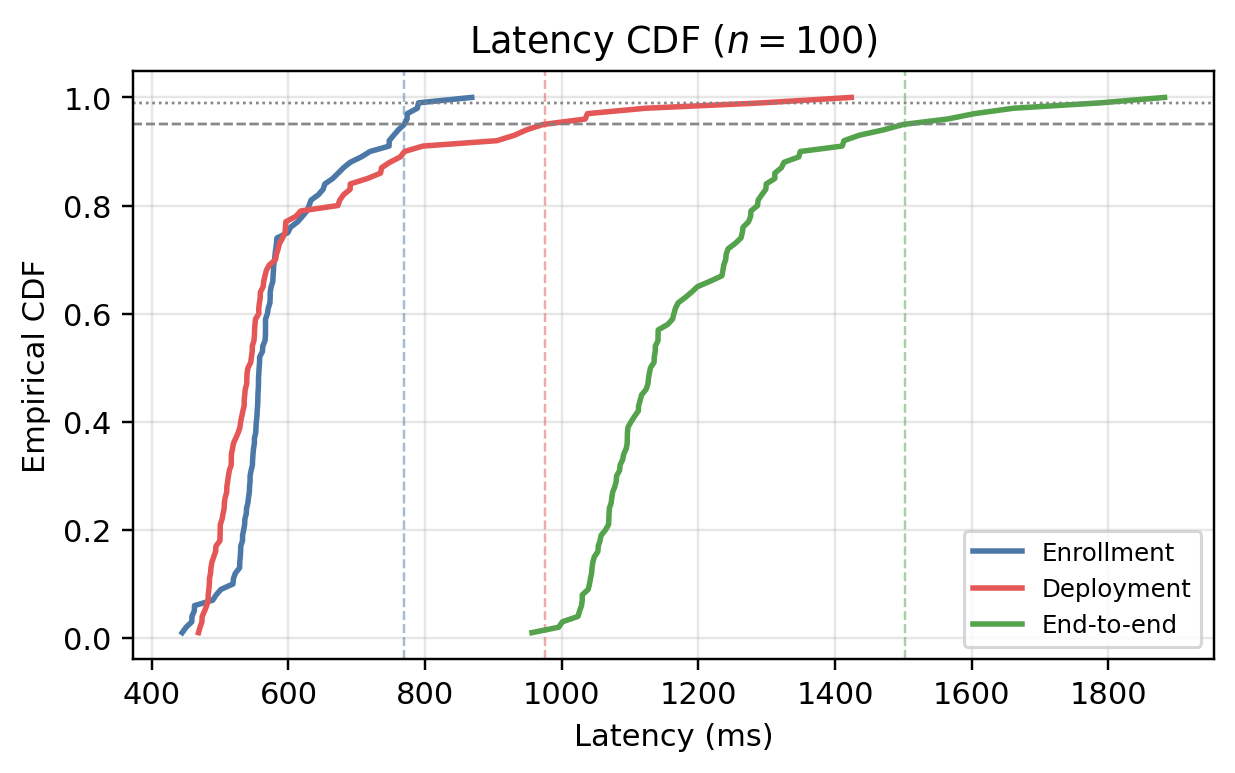
\includegraphics[width=\columnwidth,height=0.26\textheight,keepaspectratio]{figures/latency_cdf.png}
\caption{Empirical CDF of enrollment, deployment, and end-to-end latencies ($n{=}100$).}
\label{fig:latency-cdf}
\end{figure}

\subsection{Sustainability-Oriented Metrics}
\label{sec:sustainability-metrics}

\subsubsection{Southbound wire efficiency}
Application messages use a 4-byte big-endian length prefix followed by CBOR payloads. Figure~\ref{fig:wire-sizes} summarizes measured wire sizes for representative messages. Heartbeat request and acknowledgment are 6~B each; a complete enrollment round trip totals 87~B of application payload; a minimal deploy round trip (33~B WASM module) totals 90~B. At the configured 25~s heartbeat period, steady-state control traffic is $12 \times (3600/25) = 1728$~B/h per device (${\approx}$1.69~KiB/h), excluding TLS record overhead.

\begin{figure}[!htbp]
\centering
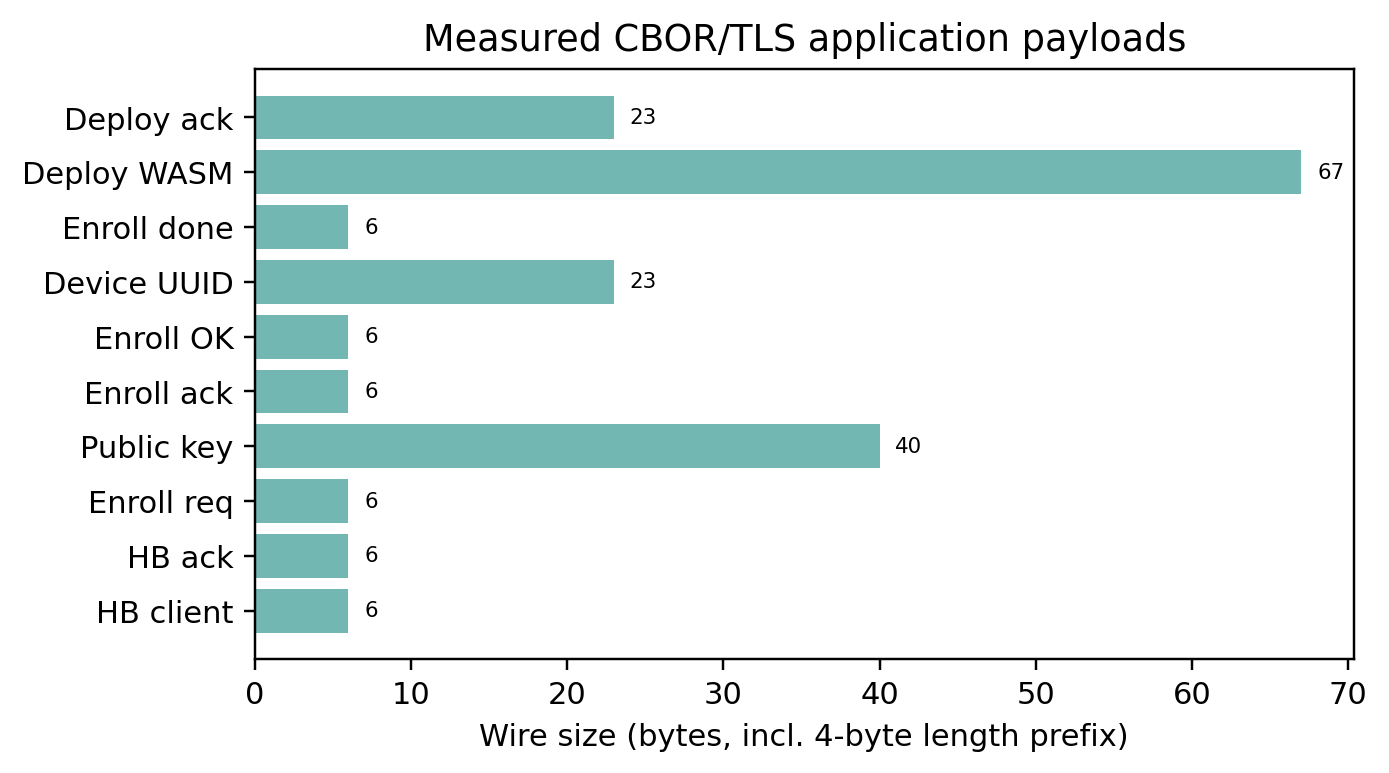
\includegraphics[width=\columnwidth,height=0.24\textheight,keepaspectratio]{figures/wire_sizes_bar.png}
\caption{Application-layer wire sizes (4-byte length prefix + CBOR) for representative protocol messages.}
\label{fig:wire-sizes}
\end{figure}

\subsubsection{Edge footprint}
The device firmware (Zephyr, network stack, WAMR, TLS/CBOR client) occupies 394~KiB of flash and 264~KiB of static RAM on the STM32F746, comfortably within the board's 1~MiB flash and 320~KiB RAM budget. The flash figure combines 393{,}980~B of code (\texttt{.text}) and 9{,}380~B of initialized data (\texttt{.data}); the RAM figure adds 260{,}818~B of \texttt{.bss}. The unstripped ELF loaded by the emulator is larger (8.0~MB) only because it retains debug symbols and section metadata that are not present in the flashed image. The benchmark WASM module is 33~B. Embedded endpoints run no kubelet, container runtime, or Linux userspace.

\subsubsection{Control-plane resources}
Figure~\ref{fig:pod-resources} reports mean Kubernetes pod usage ($n{=}5$ samples, one TLS-connected device). The gateway averaged 3.6~millicores CPU and 18.2~MiB RAM; the API server 91.0~millicores and 201.0~MiB; the application controller 44.8~millicores and 6.0~MiB. Registering up to 50 synthetic boards through the gateway HTTP registry did not increase gateway resident memory beyond 19.0~MiB, indicating lightweight per-device mediation state at the fog layer.

\begin{figure}[!htbp]
\centering
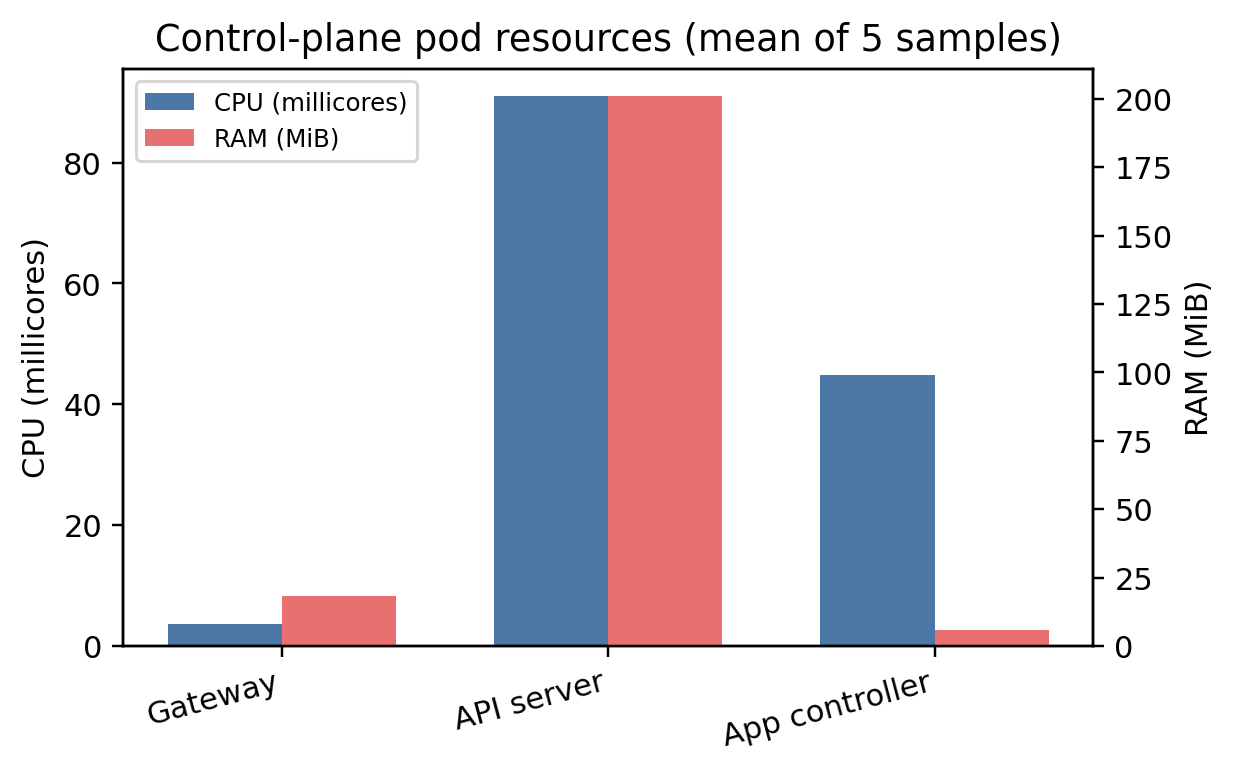
\includegraphics[width=\columnwidth,height=0.24\textheight,keepaspectratio]{figures/pod_resources_bar.png}
\caption{Mean CPU (millicores) and RAM (MiB) for control-plane pods during the sustainability measurement pass.}
\label{fig:pod-resources}
\end{figure}

\subsubsection{Architectural comparison}
Table~\ref{tab:arch-compare} contrasts gateway-mediated WASM orchestration with treating each constrained device as a Kubernetes worker. Edge Kubernetes deployments commonly require tens to hundreds of MiB of resident memory per worker for kubelet and container runtime before user workloads~\cite{kubernetes}. Our design concentrates orchestration in a shared gateway (${\approx}$18~MiB measured) while keeping cluster agents off the device.

\begin{table}[t]
\centering
\caption{Orchestration model comparison.}
\label{tab:arch-compare}
\footnotesize
\setlength{\tabcolsep}{3pt}
\begin{tabular}{p{0.22\linewidth} p{0.34\linewidth} p{0.34\linewidth}}
\toprule
\textbf{Aspect} & \textbf{Device as K8s worker} & \textbf{Gateway-mediated WASM edge} \\
\midrule
Edge runtime & kubelet + container runtime + OS & Zephyr + WAMR (394~KiB flash, 264~KiB RAM) \\
Edge cluster agent RAM & 100--350~MiB per node (literature) & none on device \\
Steady control traffic & CRI/container probes & 1728~B/h per device \\
Fog mediation RAM & per-node agent & 18.2~MiB shared gateway \\
\bottomrule
\end{tabular}
\end{table}

\FloatBarrier
